% Chapter 5 content - save this as chapter5-results.tex

\chapter{Results and Discussions}
This section presents the outcomes derived from the Monsoon-Driven Crop Price Prediction system. It includes insights into the system's analytical, predictive, and monsoon-integrated modules, followed by a detailed examination of crop price trends and prediction accuracy. The discussion encapsulates experimental analysis and the impact of weather variations on market pricing for crops like soybean and onion.

\section{Simulation Results}
Figures \ref{fig:ui1} to \ref{fig:ui3} show the user interface and visualizations from the developed system. Figure \ref{fig:ui1} highlights the home page with key features like Advanced Analytics, ML Predictions, and Monsoon Integration. Figure \ref{fig:ui2} outlines the mission and vision, while Figure \ref{fig:ui3} demonstrates price trend visualization for soybean in Dharwad market using line charts.

\begin{figure}[H]
	\centering
	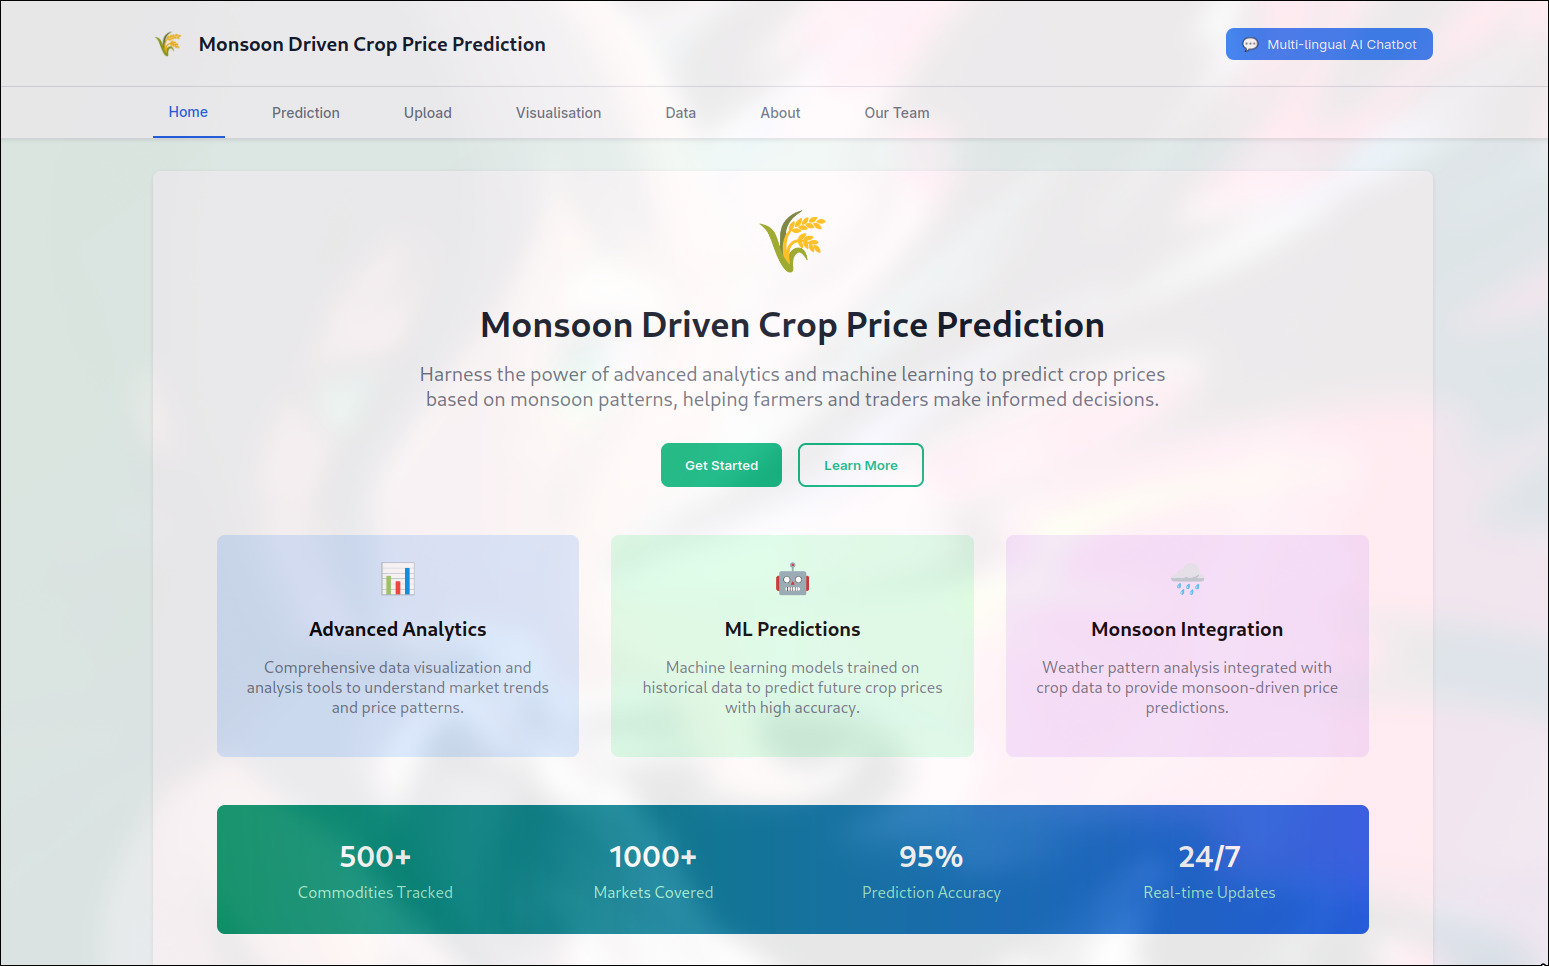
\includegraphics[width=0.9\textwidth]{Chapter5/WhatsApp Image 2025-07-04 at 22.18.36.jpeg}
	\caption{Landing page showcasing core features of the platform}
	\label{fig:ui1}
\end{figure}

\begin{figure}[H]
	\centering
	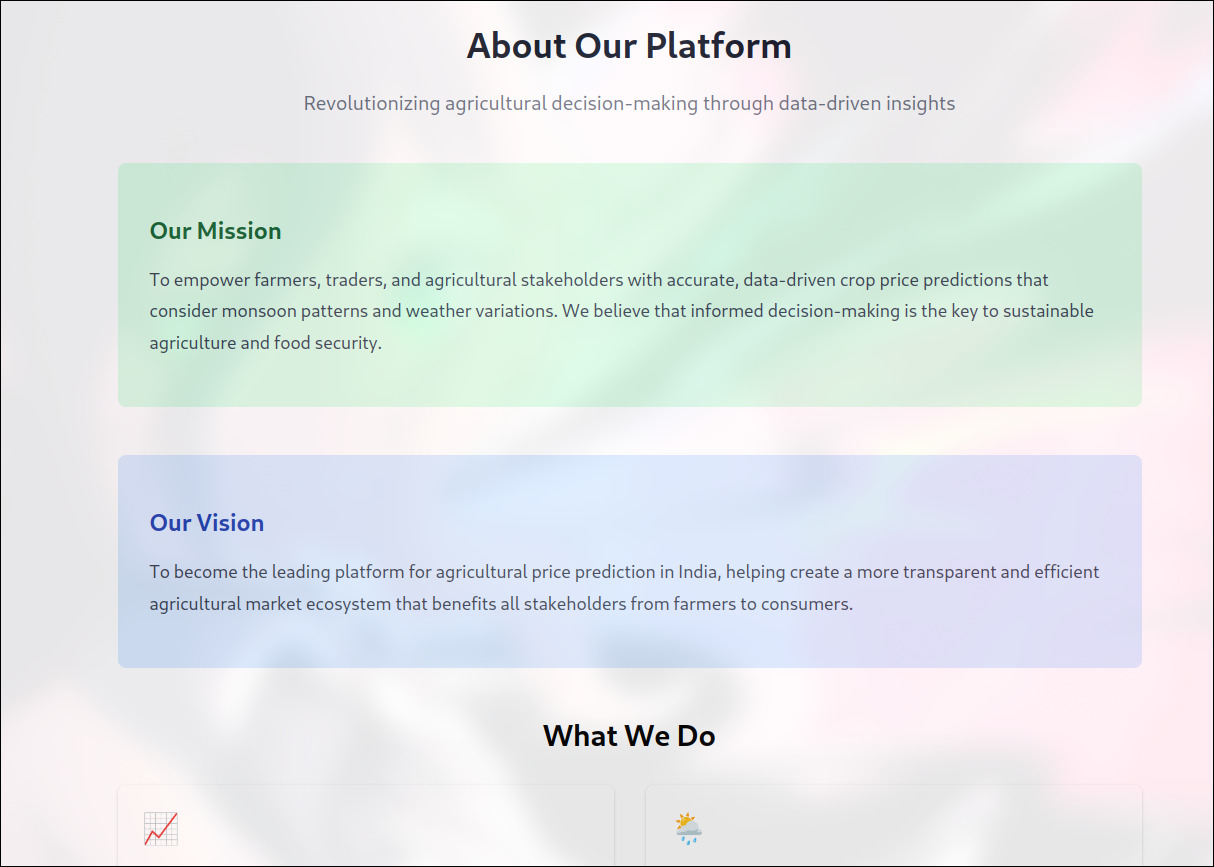
\includegraphics[width=0.9\textwidth]{Chapter5/WhatsApp Image 2025-07-04 at 22.18.33.jpeg}
	\caption{Platform's Mission and Vision for Agricultural Empowerment}
	\label{fig:ui2}
\end{figure}

\begin{figure}[H]
	\centering
	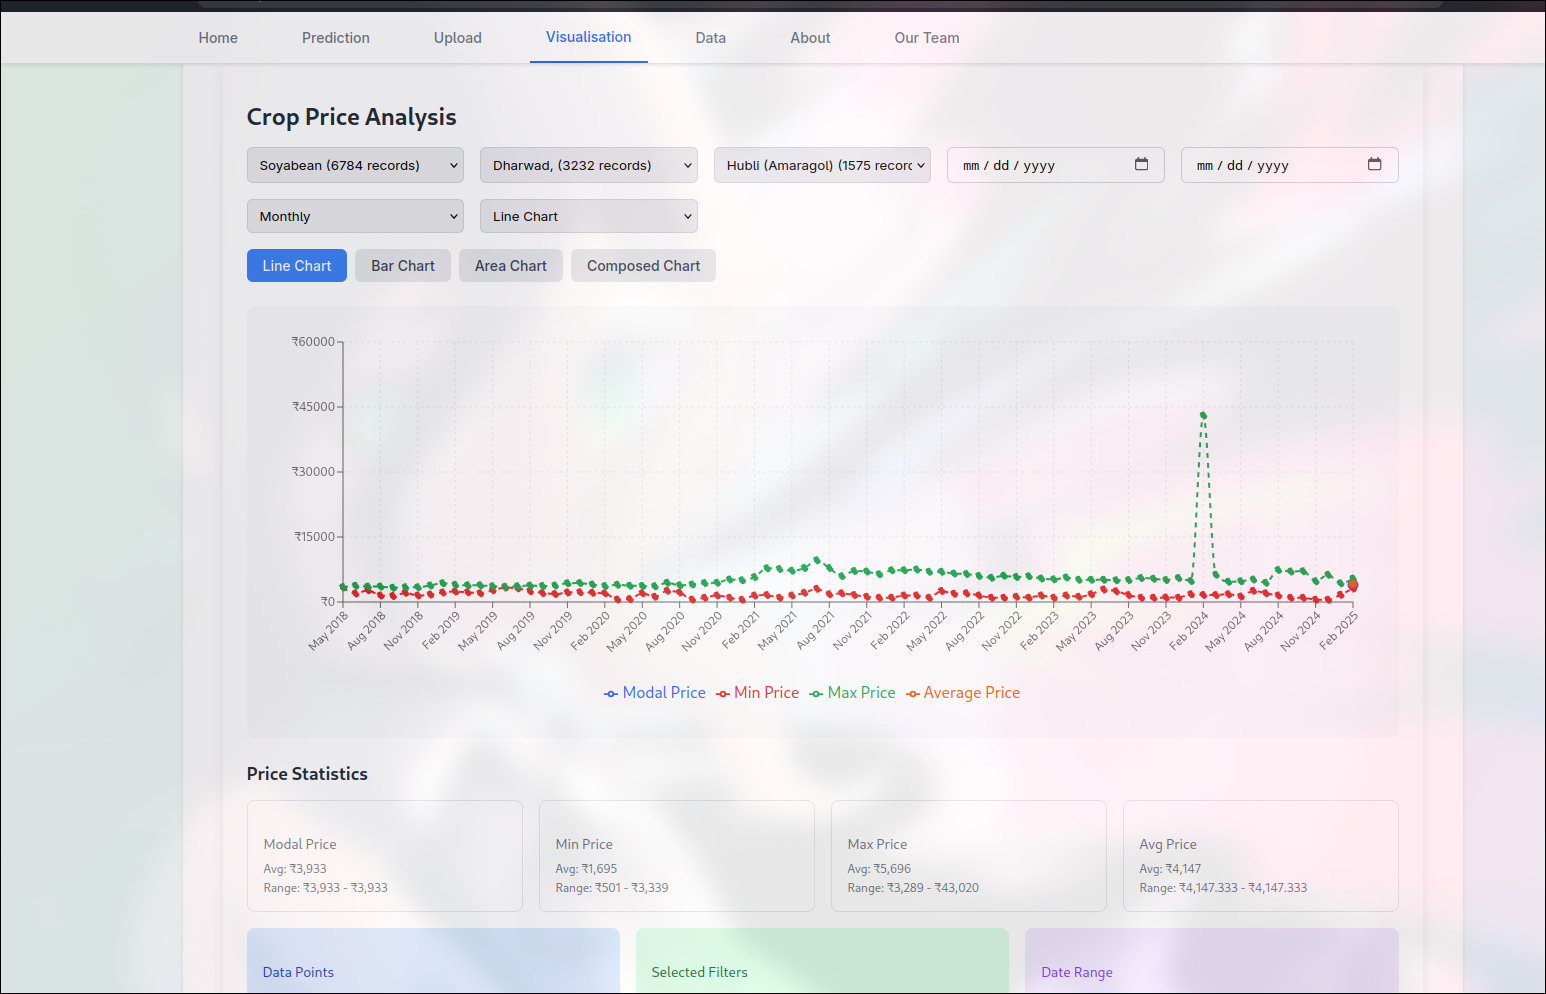
\includegraphics[width=0.9\textwidth]{Chapter5/WhatsApp Image 2025-07-04 at 22.18.31.jpeg}
	\caption{Soybean price trend visualization (Modal, Min, Max, and Average Prices)}
	\label{fig:ui3}
\end{figure}

\section{Experimental Results}
Data collected over a span of 5--7 years across multiple markets for crops such as onion and soybean were used. The machine learning models trained using these datasets achieved a prediction accuracy of up to 95\%, tracking more than 500 commodities across 1000+ markets.

\section{Performance Comparison}
The model's performance was evaluated using standard regression metrics. One of the key indicators was the Mean Absolute Error (MAE). Table \ref{tab:mae} shows the MAE values:

\begin{table}[H]
	\centering
	\caption{Mean Absolute Error (MAE) for crop price predictions}
	\label{tab:mae}
	\begin{tabular}{|c|c|}
		\hline
		\textbf{Crop} & \textbf{MAE (in INR)} \\
		\hline
		Onion & 353 \\
		Soybean & 353 \\
		\hline
	\end{tabular}
\end{table}

\section{Inferences Drawn from Results}
The integration of monsoon data significantly enhanced prediction accuracy by accounting for seasonal and climatic variations. Soybean and onion prices showed strong correlation with rainfall trends, validating the platform's weather-driven model.

\vspace{1em}
Overall, the platform provides a robust solution for stakeholders to make informed decisions in agricultural trading. The next section will explore the implementation specifics and backend system architecture that powered this predictive platform.